%=========================================================================
% sec-intro
%=========================================================================

\section{Introduction}
\label{sec-intro}

%=========================================================================
% fig-intro-dgemm.tex
%=========================================================================

\begin{figure}[h]

  \centering
  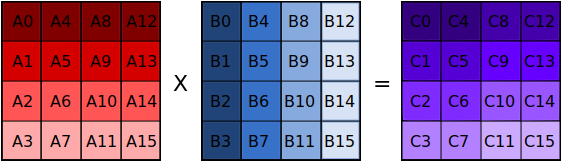
\includegraphics[width=0.7\tw]{fig-intro-dgemm.svg.pdf}

  \caption{\textbf{Double-Precision General Matrix-Matrix Multiply --}
    For simplicity, 4x4 matrices are shown with elements labeled in the
    column-major order. Rows of input matrix {\tt{A}} is multiplied with
    columns of input matrix {\tt{B}} and accumulated to generate the
    output matrix {\tt{C}}.}

  \label{fig-intro-dgemm}

\end{figure}


In this report, we explore several optimizations for improving the
performance of double-precision general matrix-matrix multiply
(DGEMM). The DGEMM algorithm, as shown in Figure~\ref{fig-intro-dgemm},
is a standard matrix multiplication between two input matrices with
double-precision floating point elements to generate an output
matrix. The serial algorithm computes elements of the output matrix
{\tt{C}} from input matrices {\tt{A}} and {\tt{B}} as follows:

\[
C_{ij} = \sum_{k=0}^{N}A_{ik}*B_{kj}
\]
\smallskip

All optimizations are implemented on top of the provided blocking
algorithm. We compare the performance of the optimizations against this
baseline. The blocking algorithm splits the matrices into and operates on
smaller blocks that are more likely to fit in the cache to better exploit
temporal and spatial locality. The high-level goals of the optimizations
explored in this assignment are to maximize hardware resource
utilization, produce more desirable memory access patterns, ameliorate
negative cache effects, and improve static analysis in the compiler.

Specifically, the following optimizations are explored in this report:

\begin{itemize}
  \item Vectorizing with SIMD extensions to maximize hardware resource
    utilization;
  \item Changing the loop ordering to produce more desirable memory
    access patterns;
  \item Copying blocks into a scratchpad in contiguous memory to
    avoid conflict misses in the cache;
  \item Experimenting with C keywords and attributes to better express
    the intent of the code to the compiler;
  \item Utilizing profile-guided optimization to maximize the benefits of
    static analysis in the compiler;
\end{itemize}
\smallskip

The proprietary Intel cross-compiler (i.e., icc) was used for all
experiments as the generated code outperforms gcc by a significant factor
for DGEMM.

\clearpage
